\chapter{INTRODUCTION}
\label{introduction}

A Virtual Private Network (VPN) provides the illusion of a local area network
(LAN) spanning a wide area network (WAN) infrastructure by creating encrypted
and authenticated, secure\footnote{For the remainder of this document, unless
explicitly stated otherwise, security implies encryption and mutual
authentication between peers.} communication links amongst participants.
Common uses of VPNs include secure access to enterprise network resources from
remote/insecure locations, connecting distributed resources from multiple
sites, and establishing virtual LANs for multiplayer video games over the
Internet.  VPNs in this context differ from others that provide ```emulation of
a private Wide Area Network (WAN) facility using IP facilities' (including the
public Internet or private IP backbones).  ''~\cite{ip_vpns}.  This style of
VPN is used to connect large sets of machines behind routers to a virtual
private WAN, whereas this dissertation focuses on the approach of connecting
individual resources into a private LAN.

As a tool enabling collaborative environments, VPNs can be useful for various
applications.  If friends and family require computer assistance and their
computer guru no longer lives nearby, the guru can remotely log into the
machine using a VPN running over the Internet despite networking constraints
between the two parties.  When traveling abroad, a user may wish that their
Internet traffic be kept private from the local network.  A VPN can be used to
route all Internet packets securely through the user's home or office network,
ensuring the user's privacy.  Many computer and video games have multiplayer
networking components that require direct connectivity.  Most of these games
rely on centralized servers for bootstrapping limiting their lfespan.  Players
of these games can continue playing through VPNs.  Small and medium businesses
may find VPNs useful for connecting desktops and servers across distributed
sites securing traffic to enterprise networked resources.  Independent
organizations that each have limited resources can combine together their
resources through a VPN to create a powerful computing grid.

The utility of the VPN described herein is motivated from Archer~\cite{archer}.
Archer consists of over 700 core resources as well as voluntary resources from
the community to provide a dynamic and decentralized grid environment for
computer architecture researchers to share and access compute cycles with each
other.  Use of centralized systems would limit the scope of Archer and require
dedicated administration, whereas existing decentralized solutions require
manual configuration of links between peers, which is beyond the scope of
Archer's target users.  Current P2P virtual network (VN) approaches either lack
scalability or proper security components to be considered VPNs.  Whereas my
approach applies naturally to such systems.

There are various VPN architectures that attempt to deal with the challenges
presented in these use cases.  In some, certain VPN approaches may work, where
others are not applicable, and in others scenarios no current VPN approach is
applicable.  In general, successful deployment and use of VPNs face the
following challenges:  

\begin{itemize}

\item OVERLAY CONFIGURATION. Peers must be able to find each other in order to
bootstrap into the overlay and to establish links with specific users inside
the overlay.

\item CONNECTIVITY. Network asymmetries motivate the use for VPNs.  One
approach is to route all traffic through a third party, but this incurs
overheads.  There also exist approaches to allow two peers behind behind NATs
to communicate directly and falling back to a relay if the two peers are behind
too restrictive networks.

\item PEER MANAGEMENT. To ensure reliability and trust, a distributed system
should employ security.  Peer management involves providing and obtaining
security credentials as well as preventing misbehaving peers from communicating
with a user's resource or removing them entirely from the system.

\item PRIVACY. The original intention for VPNs was network security,
thus all communication between peers is private.  Many VPNs only secure traffic
between hops and are thus susceptible to man-in-the-middle attacks, though
establishing end-to-end privacy can be challenging as it requires additional
out-of-band exchanges.

\item ENDPOINT CONFIGURATION. Applications transfer packets through
a network interface.  Endpoint configuration addresses the location where a
network packet is transferred through the overlay to another.

\end{itemize}

Collaborative environments can strongly benefit from a VPN that is both
user-friendly as well as scalable.  A system that is only user-friendly will
initially attract interest but frustrate them in the long run.  While systems
that lack user-friendliness will have limited user adoption.  By applying these
requirements to the aforementioned challenges leads to the following
requirements:  (1) a collaborative VPN should be easy to configure, such that
users should be able to deploy and use them without being experts in operating
systems (OSs) or networks; (2) the system should not require additional
resources to support more users; (3) adding new users and resources should be
straight-forward using approaches familiar to common users; (4) peers should be
able to connect to each other directly if and when possible; and (5) all
communication, not just hop-by-hop, should be secure.

While existing VPNs are able to meet some of these requirements, they are
unable to meet them all.  Centralized approaches (e.g.  OpenVPN~\cite{openvpn})
by their very nature require dedicated infrastructures and do not allow direct
communication between peers though when configured to do so are able to
guarantee all-to-all communication regardless NAT and firewall conditions.
Peer-to-peer (P2P) based approaches (e.g.  Hamachi~\cite{hamachi},
Wippien~\cite{wippien}, Gbridge~\cite{gbridge}, PVC~\cite{pvc}) solve the issue
of direct communication, though they are vulnerable to man-in-the-middle
attacks when session management is handled by an external provider, rely on a
central resource for the creation of VPN links, and require managed relays if
direct peer communication across NATs and firewalls fails.  Distributed
approaches (e.g., ViNe~\cite{vine}, Violin~\cite{violin}, VNET~\cite{vnet},
tinc~\cite{tinc}) require manual configuration of links between members of the
virtual network.  Existing P2P overlay approaches lack scalability
(N2N~\cite{n2n} and P2PVPN~\cite{p2pvpn}) or are difficult to configure and
lack privacy (I3~\cite{i3}).

My work culminates in a novel design and implementation of a VPN from endpoint
configuration to overlay construction and organization resulting in an
autonomic VPN that bridges the gap between user-managed VPNs and those hosted
by third-party services.  The VPN builds on top of a P2P system used to
transparently handle network asymmetries and support address allocation and
resolution.  The P2P system organizes into a structured overlay, which supports
highly scalable, distributed data sharing via a distributed hash table (DHT).
Peers search for each other by querying the DHT and then use constructs
provided by the P2P layer to form direct links or relays with remote peers.
Peer management is handled through common social networking interfaces such as
dedicated group infrastructures or relationships based upon XMMP or Facebook.
Both the VPN and the overlay are secured by a common security filter framework,
which can be bootstrapped into from existing overlays.  Finally, through
various VPN models, users and system administrators can take the same VPN
software and install it in various environments with minimal configuration
overhead.

\section{Virtual Private Network Basics}

VPNs consist of two components: clients and servers~\footnote{The definition of
a server is VPN dependent, it might be an independent infrastructure, an
overlay, or even a client in the case of P2P systems.}.  Clients discover other
clients by means of servers or overlays.  Depending on the VPN style, clients
will then either communicate with each other over this infrastructure or use it
to establish direct links with each other.  While setup may be different
amongst the various VPNs, during run time, the environment provided by a VPN
client is the same regardless of how the server or overlay is implemented.  

\begin{figure}
\centering
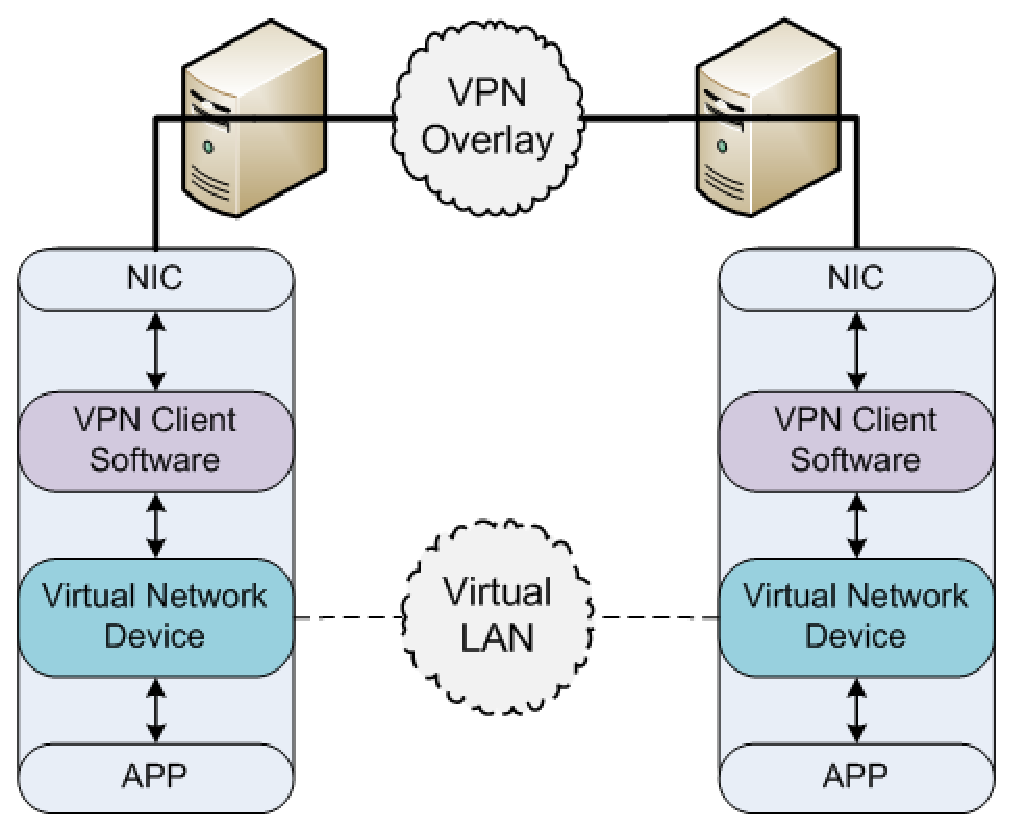
\epsfig{file=figs/vpn.png.eps, width=4in}

\caption[A typical VPN client]{A typical VPN client.  A VN device makes
application interaction with the VPN transparent.  Packets going to the VPN
destination are sent by routing rules to the VN device interfaced by the VPN
client.  The VPN client sends and receives packets from other VPN participants
via the hosts physical network device.}

\label{fig:vpn}
\end{figure}

Figure~\ref{fig:vpn} abstracts the common features of all VPNs clients, a
service and a virtual network (VN) device providing communication with the VPN
system and host integration, respectively.  During initialization, the VPN
service authenticates with the overlay by means of a centralized or distributed
service, uniquely with each peer, or some other means; then, optionally,
querying for information about the network, such as network address space,
address allocations, and domain name service (DNS) servers.  At which point,
the VPN enables secure communication amongst participants.

Clients can authenticate with the overlay using a variety of methods.  A system
can be setup quickly by using null (no) authentication or a shared secret such
as a key or a password.  Using accounts and passwords with or without a shared
secret provides individualized authentication, allowing an administrator to
block all users if the shared secret is compromised or individual users who act
maliciously.  Using unique private keys with corresponding signed certificate
provides the most secure approach because it eliminates the feasibility of
brute force attacks.  The trade-offs in the approaches come in terms of
security, usability, and management.  While the use of signed certificates
provides better security than shared secrets, certificates require more
configuration and maintenance.  Unlike passwords, certificates cannot easily be
compromised by brute force attacks.  In a system comprising of non-experts,
like university VPNs, the usual setup uses a shared secret and individual user
accounts.  Secrets can be packaged with the VPN application, so long as it is
distributed through secure channels such as authenticated HTTPS.

A VN device allows networking applications to communicate transparently over
the VPN.  The VN device provides mechanisms for injecting incoming packets into
and retrieving outgoing packets from the networking stack, enabling the use of
common network APIs such as Berkeley Sockets, allowing existing applications to
work over the VPN without modification.  While there are many different types
of VN devices, TAP~\cite{tap} stands out from the rest due to its open source
and pervasive nature.  TAP allows the creation of one or more Virtual Ethernet
and / or IP devices and is available for almost all modern operating systems
including Windows, Linux, Mac OS/X, BSD, and Solaris.  A TAP device presents
itself as a character device providing read and write operations.  Incoming
packets from the VPN are written to the TAP device and the networking stack in
the OS delivers the packet to the appropriate socket.  Outgoing packets from
local sockets are read from the TAP device.

VN devices are no different than any other network device.  They can be
configured manually through command-line tools or OS' APIs or dynamically by
the universally supported dynamic host configuration process
(DHCP)~\cite{dhcp0, dhcp1}.  Upon the VN device obtaining an IP address, the
system adds a new rule to the routing table that directs all packets sent to
the VPN address space to be directed to the VN device.  Packets read from the
TAP device are encrypted and sent to the overlay via the VPN client.  The
overlay delivers the packet to another client or a server with a VN stack
enabled.  Received packets are decrypted, verified for authenticity, and then
written to the VN device.  In most cases, the IP layer header remains
unchanged, while VPN configuration determines how the Ethernet header is
handled.

\section{Computer Network Architectures}

All models for computer communication in distributed systems fall under two
categories:  centralized and decentralized.  They can be further divided into
hybrid systems with centralized session management and decentralized
communication and self-configuring, dynamics P2P systems.  Thus the
architectures commonly used for implementing VPN systems are centralized
organization and communication, centralized organization and decentralized
communication, decentralized with manual organization, and decentralized with
automatic organization.

Centralized organization and communication systems consist of clients and
servers with all distributed peers both locally and remote are clients
discovering and connecting, or organizing, through a dedicated centralized
resource. Clients never communicate with each other directly only, but rather
every message between two clients must traverse the server.  For instance, most
online social networks (OSNs) are representative of these type of systems.
Users of OSNs like Facebook~\cite{facebook} and MySpace~\cite{myspace}
communicate through centralized environments never directly to each other's
computers.  OpenVPN~\cite{openvpn} represents this domain in VPNs.  These
systems rely on on dedicated resources.  In the situation that a server goes
offline or becomes overwhelmed by the clients, the system is rendered useless.

Centralized organization and decentralized communication systems include the
first set of popular P2P systems, such as the original Napster, Kazaa, and VPNs
like Hamachi~\cite{hamachi}.  Similar to the client-server model, clients
connect to a server to find other clients, though instead of communicating
through the server, the clients form direct connections with each other.  These
approaches are limited by network address translation (NAT) and firewalls that
may prevent peers from communicating with each other.  In these cases, the
central server may act as a relay allowing the two clients to communicate
through it.  Unlike systems using centralized communication, these systems are
less susceptible to being overwhelmed by client traffic and even if the server
goes offline existing client links remain active, though new connections cannot
be established.

Systems employing decentralized communication with manual organization address
the issues of a central system going offline, because clients are configured to
connect to any number of distributed servers forming an overlay.  In these
systems, servers are explicitly configured to communicate with other servers.
Though this approach improves upon the issues inherent with completely
centralized architectures, if a site goes offline any systems communicating
through it will no longer be connected to the rest of the system until the
administrator creates additional links or the site becomes active again.
Clients in these systems do not typically form direct links with each other,
rather they route packets through the overlay.  This approach has been used to
create scalable VPNs, like ViNe~\cite{vine}, VNET~\cite{vnet},
Violin~\cite{violin}, and Layer 2 Tunneling Protocol based VPNs~\cite{l2tp}.

In decentralized communication with automatic organization-based, there is no
distinction amongst peers as they act as both client and servers, i.e., a P2P
system or overlay.  P2P systems are usually distributed with a list of common
peers.  Peers attempting to bootstrap into the P2P overlay randomly selects
peers on this list until it is able to connect with one.  This connection is
then used to form connections with other peers currently in the overlay.  The
overlay can be organized in two different forms: randomly or deterministically
creating unstructured or structured overlays, respectively.  In an unstructured
overlay, links are formed arbitrarily, thus a peer searches for another peer by
broadcasting the message or using stochastic techniques.  In structured
overlays, peers organize into topologies by deterministically forming
connections with peers nearby in the overlay address space creating structures
such as ring and hybercubes.  Peers can be found deterministically using greedy
routing approaches in usually $O(\log(N))$ time.  Gnutella~\cite{gnutella} file
sharing system and Skype~\cite{skype} are popular examples of unstructured
systems, while P2PSIP~\cite{p2psip} and distributed hash tables
(DHTs)~\cite{chord} are popular in structured systems.  The challenges to
unstructured systems is finding data objects in reasonable amount of time,
while structured systems suffer when large amount of peers join or leave the
system, known as churn~\cite{opendht}.  In general, both approaches are
difficult to secure due to their typical application.  When used in private
environments though, they have been shown to be very useful, exemplified by
Dynamo~\cite{dynamo} or BigTable~\cite{bigtable}.

This dissertation uses structured overlays as the foundation in building
scalable, decentralized VPNs, the following section reviews structured
overlays.

\section{Structured Overlays}

Structured P2P overlays provide distributed querying systems with guaranteed
search time based upon the organization of the structure though typically
within $O(\log(N))$, in contrast to unstructured systems, which rely on global
knowledge/broadcasts, or stochastic techniques such as random
walks~\cite{unstructured_v_structured}.  There exists a plethora of structured
systems found both in research and in available applications~\cite{pastry,
chord, symphony, kademlia, can, brunet}.  In order to obtain guaranteed search
time, structured systems self-organizing into well defined topologies, such as
a ring (pictured in Figure~\ref{fig:ring_overlay}) or a hypercube.  Peers
joining an overlay typically follow these abstracted steps:

\begin{figure}
\centering
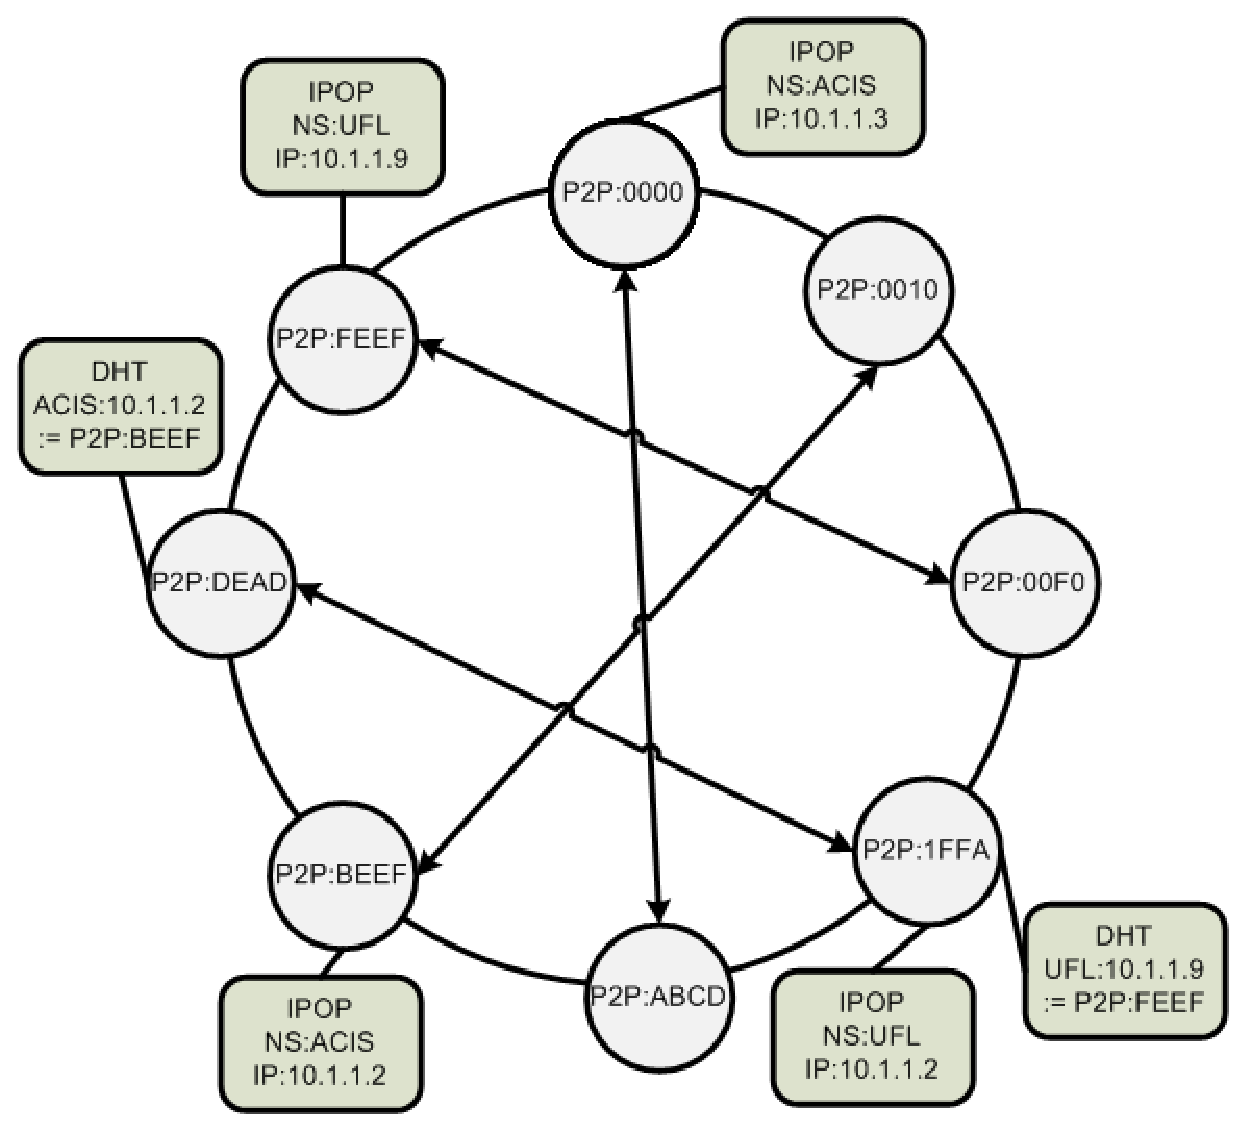
\epsfig{file=figs/ring.eps, width=6in}
\caption{1-D ring structured overlay}
\label{fig:ring_overlay}
\end{figure}

\begin{enumerate}

\item generate or obtain a unique identification number (node ID) within the
overlay's address space, usually on the order of 128-bits to 256-bits;

\item attempt to connect to one or more random addresses from a pre-shared list
of well-known endpoints, dedicates resources from a service provider or users
with high uptime;

\item become connected to at least one peer in this list (leaf connection,
bootstrap peer);

\item find the set of peers in the address space closest to the node's ID;

\item establish connections or exchange connection information with those peers
(neighbor or near connections);

\item and finally connect to other nodes in the overlay outside the set of near
connections to enable quickly traversing the address space (shortcut or far
connections).

\end{enumerate}

All nodes are required to have a unique node ID.  Address collisions confuse
the overlay, potentially fragmenting it and other potential abnormal behaviors,
and of course, one or both of the nodes will not be able to properly connect to
the overlay.  Furthermore, having uniformly distributed node IDs enhances the
capability of the shortcut connections in order to better traverse the overlay.
To obtain a good distribution of node IDs, either a central server can provide
the ID ensuring or each node independently of others can use a
cryptographically strong random number generator.  The former approach can be
used to create a trusted overlay by having the third-party sign each node
IDs~\cite{secure_routing}.

In a ring, each node must be connected to closest neighbors in the node ID
address space, that is the node immediately before and after it; optimizations
for fault tolerance suggest that for ring topologies the amount should be at
least 2 and up to $\log(N)$ on both sides.  Consider the case when there is
overlay disconnectivity potentially due to churn; a peer receives a packet but
cannot route it closer to the destination than itself because it does not have
a connection with that peer.  The message may either be locally consumed or
thrown away never arriving at its intended destination.  Increasing the number
of near neighbor peers reduces the likelihood chances of packets being lost due
to churn, especially if peers leave suddenly without warning.

As mentioned, shortcuts or far connections enable efficient routing in
ring-based and similarly designed structured overlays.  The various shortcut
selection methods include: maintaining large tables without using connections
and only verifying usability when routing messages~\cite{pastry, kademlia},
maintaining a connection with a peer at specific locations in the P2P address
space~\cite{chord}, or using locations drawn from a harmonic distribution in
the node address space~\cite{symphony}.

Structured overlays support decentralized query systems that can be used to
build distributed data structures such as a distributed hash table (DHT) by
mapping keys via a hash function to P2P IDs in an overlay.  The data associated
with the key is then stored at the node closest to the P2P id of the key and
for fault tolerance can be stored by other nodes nearby or more keys can be
generated by recursively hashing the original key.  Using the DHT primitives,
Past~\cite{past} and Kosha~\cite{kosha} projects have designed more complex
distributed data stores.

The actual mechanism for querying nodes or routing in a P2P overlay can be
either iterative or recursive.  In iterative routing, the querying node
iteratively contacts nodes closer and closer to the address until finding the
closest node at which point it makes the request directly to that node.  In
more detail, the querying node directly queries the node closest to the
destination, that node returns back one or more network (IP) and P2P addresses
of closer peers, the querying node queries these peers, and the process
continues until determining there exists no closer node.  Alternatively in
recursive routing, a querying peer sends the message to the peer closest to the
destination from its perspective, that peer repeats the process until the
message has arrived at the closest peer to the address or the destination.
Compared to recursive routing, iterative can be implement more easily though
with considerable overhead as each overlay query will cause $\log(N)$
connections to form.  NATs further complicate the use of iterative routing as
peers attempting to connect with another peer behind a NAT will need the
assistance of a third-party; whereas, recursive routing maintains active
connections and messages seamlessly traverse NAT links and non-NAT links since
the connections are established prior to message transmission.

\section{Network Asymmetries}

Naive P2P systems assume network symmetry, that is any peer can communicate
directly with any other peer using the underlying infrastructure.  Unless the
software is run inside a LAN or an environment where the network topology is
well controlled and defined, symmetry cannot be guaranteed.  P2P used in wide
area systems often relies on the Internet.  Besides the potential routing
outages on the Internet, significant amount of resources which are not directly
accessibe are connected to it.  The issue is only further pressed by the
current means of connecting to the Internet: Internet Protocol (IP) version 4
(IPv4) with its limited address space of only $2^{32}$ (approximately 4
billion).  With the Earth's population at over 6.8 billion and each individual
potentially having multiple Internet-capable devices, these limitations become
more apparent.

Currently the two approaches addressing IPv4 limitations are:  the use of
NATs to enable many machines and devices to share a single IP address but
preventing bidirectional connection initiation and IPv6 which supports
$2^{128}$ addresses.  The use of NATs, as shown in Figure~\ref{fig:nat},
complicates the bootstrapping of P2P systems as it prevents peers from simply
exchanging addresses with each other to form connections, as the addresses may
not be public.  In addition, firewalls may prevent peers from receiving
incoming connections.  Thus, while the eventual widespread use IPv6 may
eliminate the need for address translation, it does not deal with the issue of
firewalls preventing P2P applications from communicating as well as routing
outages, and it is not clear that IPv6 users will not continue to rely on
NAT/firewall devices to provide a well-defined boundary of isolation for their
local networks.

\begin{figure}
\centering
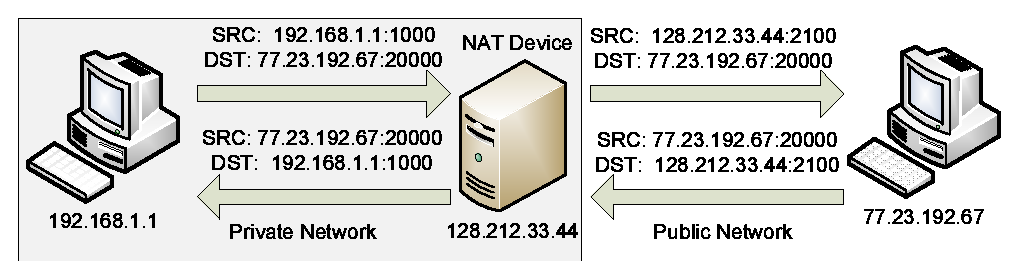
\epsfig{file=figs/NAT.eps, width=5in}
\caption[A typical NAT interaction]{A typical NAT interaction. The peer behind
a NAT has a private address.  When the packet is sent through the NAT, the NAT
translates the source information into a public mapping, keeping the original
source information so that if a packet from the remote peer comes back, it can
be translated and delivered to the original source.}
\label{fig:nat}
\end{figure}

When a machine, \textit{A}, behind a typical NAT, \textit{B}, sends out a
packet to an Internet host, \textit{C}, the NAT device translates the packet so
that it appears it is coming from the NAT device making the NAT device a
gateway.  When the packet is sent from \textit{A} to \textit{C}, the source and
destination are listed as $IP:port$ pairs, where the source and destination are
$IP_A:Port_A$ and $IP_C:Port_C$, respectively.  \textit{A} forwards the packet
to \textit{B} who transforms the source from $IP_A:Port_A$ to $IP_B:Port_B$,
where $Port_A$ may or may not be equal to $Port_B$.  This creates a NAT mapping
so that incoming packets from $IP_C:Port_C$ to $IP_B:Port_B$ are translated and
forwarded to $IP_A:Port_A$.

There are a handful of recognized NAT devices as presented in~\cite{stun,
p2p_nats_rfc}.  The following list focuses on the more prevalent types:

\begin{itemize}

\item FULL CONE. All requests from the same internal IP and port are mapped to
a static external IP and port, thus any external host can communicate with the
internal host once a mapping has been made.

\item RESTRICTED CONE. Like a full cone, but it requires that the internal host
has sent a message to the external host before the NAT will pass the packets.

\item PORT RESTRICTED CONE. Like a restricted cone, but it requires that the
internal host has sent the packet to the external hosts specific port, before
the NAT will pass packets.

\item SYMMETRIC. Each source and destination pair have no relation, thus only a
machine receiving a message from an internal host can send a message back.

\end{itemize}

Of the various scenarios involving peers and NATs, so long as one peer is on
any of the cone NATs and there are no firewalls, it can receive incoming
connection requests.  Challenges to this approach exist when firewalls are
introduced or both peers are behind symmetric NATs.  Firewalls may traffic that
would otherwise allow NAT traversal, whereas symmetric NATs require complex
mechanisms in an attempt to have incoming connection requests.  These types of
systems typically rely on a third-party to pass messages between the peers.

\section{Contributions}

Applying the challenges listed in the introduction to collaborative
environments the resulting requirements are self-configuring environments
enabling even non-experts to setup, deploy, and manage their own VPNs; peers
should communicate with each other directly when possible or through efficient
indirect paths when constrained; and the system should be reliable and ensure
the privacy of its users To address these requirements, I propose a novel
GroupVPN using structured overlays consisting of the following novel
contributions:

SECURE OVERLAYS. Typical overlays are secured using heuristics that limit the
effects of malicious users; however, Skype is not.  Challenges of using secure
sessions for instituting trust or security into an overlay depends on the
communication path ways.  If the goal for the system is to support asymmetries
on the network, then the system will have to make significant use of datagram
technologies.  This work proposes a unique filter mechanism to support
encrypting any form of communication between two parties and examines the
overheads of deploying it in simulated and real environments.

BOOTSTRAPPING AD-HOC, DECENTRALIZED SYSTEMS. Secure overlays present a
challenge when there will be a one to one mapping between overlay and VPN in
order to securely isolate a VPN.  This stems from the fact that at any given
time, peers may or may not be connected to the overlay.  When used in small
groups, most or all members may be behind NATs or remain online for short
periods of time.  Creating a situation, where not a single user on a publicly
addressable resource will be online, limiting the use of private overlays.  To
address this issue, I propose the reusing of public free-to-join overlays to
bootstrap into a private overlay.  Peers use the public overlay to find each
other and exchange connection information using secure messages.  Only peers
with appropriate security credentials are able to join the private overlay.

DECENTRALIZED RELAYS. In collaborative environments, most peers are behind NATs
and potentially firewalls as well.  While in general most NATs are traversable
through existing approaches, not all are.  Firewalls only complicate the
matter.  While these peers may be able to communicate through the overlay, as
the overlay grows, this latency can become a hindrace to usability and
interactivity.  To improve this situation, I propose the creation of autonomic
2-hop relays between the peers.

USING SOCIAL INFRASTRUCTURES FOR MANAGEMENT AND DISTRIBUTION OF SECURITY
CREDENTIALS. In order to simplify the management and access to a VPN, this
component explores the use of social networks in terms of both groups and peers
to facilitate trust establishment for a VPN.  Beyond the obvious contribution
of uniquely using social networks to establish VPN trust, this shows how
systems can leverage trust in an existing environment for use it in another,
which has significant usage when the user interface complexity between the two
differs significantly.

SELF-CONFIGURING VPN ARCHITECTURES. Many existing VPN approaches require the
users to setup their environment and do not provide a plug and play system.  In
addition, different environments call for different types of VPNs, explicitly,
individual users connect via their own VPN connections, while clusters may
benefit from a shared VPN or may desire fault tolerance of having many but do
not want the communication overhead when talking to VPN peers on the LAN.  I
address this issue with a self-configuring VPN approach that can be applied to
various local environments scaling from a single computer to many.

OVERLAY COMMUNICATION MODELS. In my experience, when using the overlay based
connections, performance suffers due to being processed by the overlay's state
machine.  I will work towards addressing this issue by investigating different
models for using overlays to establish direct communication: communicating
through the overlays state machine, bypassing the overlay's state machine but
reusing its connection management, and creating links separate from the
overlay.

P2P VPN ENABLED INTERNET TRAFFIC TUNNELING. When in insecure environments such
as browsing private information in a coffee shop, users may desire to prevent
local users and administrators from sniffing their traffic.  Traditional VPNs
support this behavior, but the approach is difficult to implement in P2P
systems due to their dynamic nature.  Currently, no decentralized VPN supports
the ability to perform this behavior.  I propose a method that not only works
for decentralized and P2P systems but ensures a greater level of security than
existing approaches by securing other non-VPN communication between the peer
and gateway resources.

AD-HOC, DISTRIBUTED SYSTEMS. The value in a complex system like the one
proposed herein can be realized when tied together for the creation of ad-hoc,
distributed systems.  The type of system focused on in this paper is a grid.
While there are many grid topologies, approaches that share resources amongst
users and even most that are used by a single user require a user with
expertise in operating systems, networks, and middleware.  This theis shows by
means of P2P and a P2P VPN methods and techniques that can be used to create a
trusted, ad-hoc, distributed grid that requires little if any expertise in the
underlying technology being utilized.

DECENTRALIZED SOCIAL NETWORKS. Traditional approaches to social networks, such
as Facebook and MySpace, requires trust in a third-party entity.  These
third-parties mine users information for advertisements, potentially violating
user's privacy.  This dissertation presents a decentralized social network that
addresses real problems by taking advantage of the P2P system described herein
by providing each user in a social network their own private overlay whose
members constitute the friends of that individual.

BUILT-IN SELF-SIMULATION. Most research paths begin by implementing a model,
followed by a simulator, and then finally deployable software.  This may cause
two or three implementations of the same concept.  Unfortunately each new
iteration requires reimplementation of the same algorithms and state machines.
So while the simulation software shows no faults, during the transition from
simulation to deployment, bugs are introduced, potentially slowing down
progress and making it difficult to transition between the two.  My approach
integrates the two in order to seamlessly transition code directly between the
two, reducing development times and easing bug tracking and fixing.

IMPROVED MODELS FOR DIRECT CONNECTION ESTABLISHMENT.  Originally, direct links
in the P2P VN were based upon packet flow passing a threshold.  Through the use
of profiling real systems and published results of Internet behavior, I have
concluded that this model does not scale well and have design and implemented a
model that satisfactorily solves this problem.

The rest of this dissertation is organized as follows.  Chapter~\ref{chap:vpns}
overviews existing VN and VPN approaches and discusses configuration and
organization of the VPN including end-point configuration.  In
Chapter~\ref{chap:bootstrapping}, I review the challenges to bootstrapping
overlays and present my solution that reuses existing overlays to bootstrap
smaller, ad-hoc overlays.  This leads into Chapter~\ref{chap:security}, which
discusses security issues in structured overlays and addresses the means to
boot private and secure VPNs.  Chapter~\ref{chap:extensions} covers extensions
to the VPN based upon practical demands and experiences.
Chapters~\ref{chap:gridappliance} describes the Grid Appliance, the target
application for my research.  Chapter~\ref{chap:spo} presents a proposed idea
on how to use the technology discussed thus far to create a decentralized
online social network.  Finally, I conclude in Chapter~\ref{chap:conclusion} by
discussing the value in my contributions and challenges that were revealed but
not address in this body of work.
